\begin{tabular}{|c|c|c|c|c|}
  \hline
  Funktion & $x_0$ & $T_{\infty}$ & Bedingungen & Erste Terme \\
  \hline
  $\sin(x)$ & $0$ & $\sum_{n=0}^{\infty}(-1)^n \frac{x^{2n+1}}{(2n+1)!}$ & & $x - \frac{x^3}{6} + \frac{x^5}{120} - \frac{x^7}{5040} + \frac{x^9}{362880} \ldots$ \\
  \hline
  $\cos(x)$ & $0$ & $\sum_{n=0}^{\infty}(-1)^n \frac{x^{2n}}{(2n)!}$ & & $1 - \frac{x^2}{2} + \frac{x^4}{24} - \frac{x^6}{720} + \frac{x^8}{40320} \ldots$ \\
  \hline
  $\tan(x)$ & $0$ & $\sum_{n=1}^{\infty} \frac{B_{2 n}(-4)^n\left(1-4^n\right)}{(2 n) !} x^{2 n-1}$ & & $x + \frac{x^3}{3} + \frac{2x^5}{15} + \frac{17x^7}{315} + \frac{62x^9}{2835} \ldots$ \\
  \hline
  $\arccos(x)$ & $0$ & $\frac{\pi}{2} - \arcsin(x)$ & $|x|<1$ & $\frac{\pi}{2}-\left(x+\frac{x^3}{6}+\frac{3 x^5}{40}+\frac{5 x^7}{112}+\frac{35 x^9}{1152}+\cdots\right)$ \\
  \hline
  $\arcsin(x)$ & $0$ &  & $|x|\leq1$ & $x+\frac{x^3}{6}+\frac{3 x^5}{40}+\frac{5 x^7}{112}+\frac{35 x^9}{1152}+\cdots$ \\
  \hline
  $\arctan(x)$ & $0$ & $\sum_{n=0}^{\infty}(-1)^n \frac{1}{2n+1} x^{2n+1}$ & $|x|\leq1$ & $x - \frac{x^3}{3} + \frac{x^5}{5} - \frac{x^7}{7} + \frac{x^9}{9} \ldots$ \\
  \hline
  $e^{x+c}$ & $0$ & $\sum_{n=0}^{\infty} \frac{x^n}{n!}$ & & $1 + x + \frac{x^2}{2} + \frac{x^3}{6} + \frac{x^4}{24} \ldots$ \\
  \hline
  $\ln(x)$ & $1$ & $\sum_{n=1}^\infty \frac{(-1)^{n+1}}{n}(x-1)^n$ & $0 < x \leq 2$ & $(x-1) - \frac{(x-1)^2}{2} + \frac{(x-1)^3}{3} - \frac{(x-1)^4}{4} \ldots$ \\
  \hline
  $\ln(1+x)$ & $0$ & $-\sum_{n=1}^{\infty} \frac{x^n}{n}$ & & $x - \frac{x^2}{2} + \frac{x^3}{3} - \frac{x^4}{4} + \frac{x^5}{5} \ldots$ \\
  \hline
  $\sqrt{x+1}$ & $0$ & $\sum_{n=0}^{\infty} \binom{\frac{1}{2}}{n} x^n$ & & $1 + \frac{x}{2} - \frac{x^2}{8} + \frac{x^3}{16} - \frac{5x^4}{128} \ldots$ \\
  \hline
  $\frac{ax}{(b-x)^2}$ & $0$ & $\sum_{n=1}^{\infty} \frac{n \cdot x^n }{b^{n+1}}$ & & $\frac{ax}{b^2} + \frac{2ax^2}{b^3} + \frac{3ax^3}{b^4} + \frac{4ax^4}{b^5} + \frac{5ax^5}{b^6} \ldots$ \\
  \hline
  $\frac{1}{x}$ & $1$ & $\sum_{n=0}^{\infty} (-1)^n (x-1)^n$ & $x > 0$ & $1 - (x-1) + (x-1)^2 - (x-1)^3\ldots$ \\
  \hline
  $a^x$ & $0$ & $\sum_{n=0}^{\infty} \frac{(\ln a)^n}{n!} x^n$ & $a > 0$ & $1 + (\ln a)x + \frac{(\ln a)^2 x^2}{2} + \frac{(\ln a)^3 x^3}{6} + \ldots$ \\
  \hline
  $\frac{1}{x^2+1}$ & $0$ & $\sum_{n=0}^\infty (-1)^n x^{2n}$ & & $1 - x^2 + x^4 - x^6 + x^8 - x^{10} \ldots$ \\
  \hline
  $\frac{1}{1-x}$ & $0$ & $\sum_{n=0}^{\infty} x^n$ & $|x| < 1$ & $1 + x + x^2 + x^3 + x^4 + x^5 + \ldots$ \\
  \hline
\end{tabular}

\begin{table}[H]
\begin{tabular}{|c|c|c|c|} 
\hline
Objekt & Bereich & Inhalt & Schwerpunkt\\ \hline
  $\frac{1}{2}$-Scheibe &    $y>0$       &   $\frac{R^2 \pi}{2}$             &  $(0,\frac{4R}{3\pi})$           \\ \hline
  $\frac{1}{4}$-Scheibe     &   $x>0,y>0$         &              $\frac{R^2 \pi}{4}$ &    $(\frac{4R}{3\pi},\frac{4R}{3\pi})$         \\ \hline
   $\frac{3}{4}$-Scheibe    &      $y>0 \vee (x<0 \wedge y<0)$      &     $\frac{3R^2 \pi}{4}$            &    $(-\frac{4R}{9 \pi},\frac{4R}{9 \pi})$         \\ \hline
   $\frac{1}{2}$-Kugel &   $z>0$    &        $\frac{2 R^3 \pi}{3}$    & $(0,0,\frac{3R}{8})$                         \\ \hline
\end{tabular}
\end{table}


\begin{table}[H]
\resizebox{\linewidth}{!}{%
\begin{tabular}{lllll}
$\int \cos^{a}\sin^{b}$ & $b=0$ & $b=1$ & $b=2$ & $b=3$ \\
\hline
$a=0$ & $C$ & $-\cos(x)$ & $\frac{1}{2}(x-\sin (x) \cos (x))$ & $\frac{1}{12}(\cos (3 x)-9 \cos (x))$ \\
$a=1$ & $\sin(x)$ & $-\frac{1}{2} \cos ^2(x)$ & $\frac{\sin ^3(x)}{3}$ & $\frac{\sin ^4(x)}{4}$ \\
$a=2$ & $\frac{1}{2}(x+\sin (x) \cos (x))$ & $-\frac{1}{3} \cos ^3(x)$ & $\frac{1}{32}(4 x-\sin (4 x))$ & $\frac{1}{30} \cos ^3(x)(3 \cos (2 x)-7)$ \\
$a=3$ & $\frac{1}{12}(9 \sin (x)+\sin (3 x))$ & $-\frac{1}{4} \cos ^4(x)$ & $\frac{1}{30} \sin ^3(x)(3 \cos (2 x)+7)$ & $\frac{1}{192}(\cos (6 x)-9 \cos (2 x))$ \\
\end{tabular}}
\end{table}




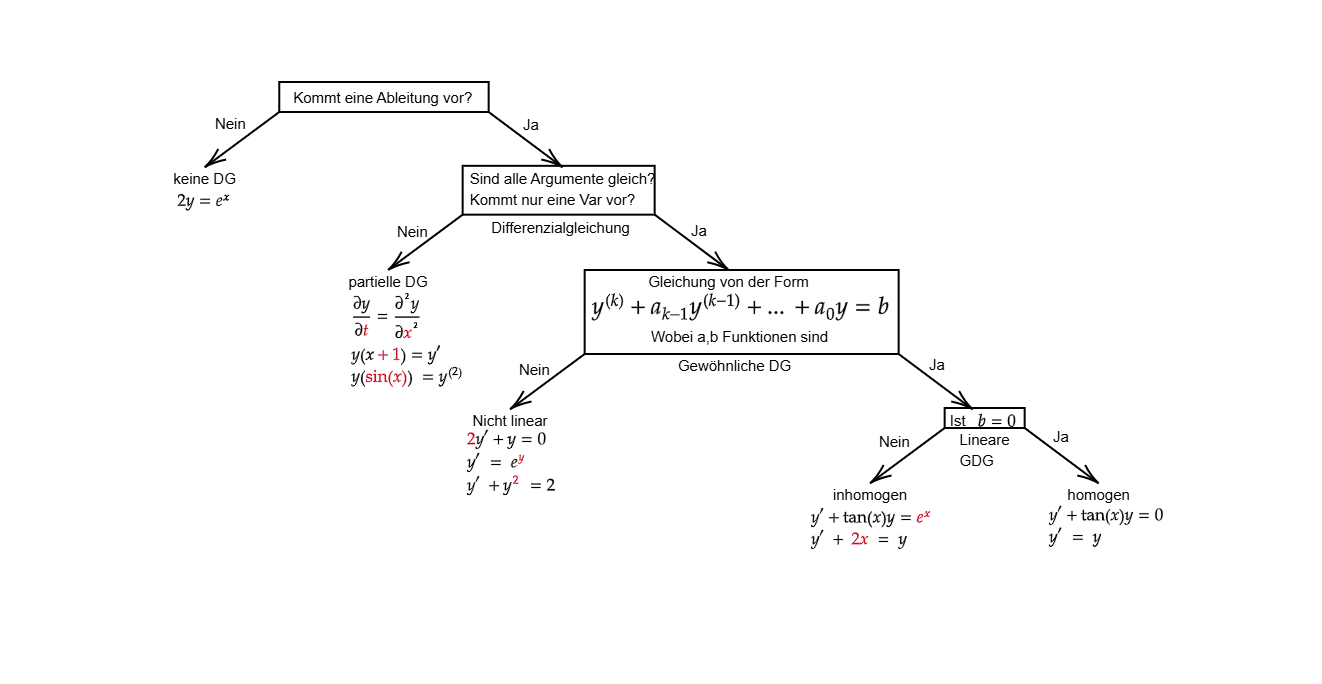
\includegraphics[scale=0.3]{build/pictures/decision_tree.png}

 

